\chapter{Reproducibility Material}\label{appendix:reproducibility}

The implementation is based on commit
\texttt{29d09aa0b14ecefe7278d201fd31cd2a96dbf5d3}, identified locally by tag
\texttt{x01-locked-20260906}. The selected PVO evaluation executable is
identified by SHA-256
\texttt{bd9b6641fb7ba57df508cf188125838474fb29a689d96d7b271a99e2a1464659}.
The SHA-256 values below identify the selected PVO configuration (internally p01),
VOCA MV-first, VOCA OF-first, and EuRoC calibration JSON files, respectively.

\begin{lstlisting}[basicstyle=\ttfamily\small]
8457ae6d36f8c137bdbf9f4dcaa29a23d480c9f2cad1bee41176c0578c27ee1b
9533b2a8f3e059bd0e46cfe6bf9fcd857b96ffe2d4839a6ff987e80e4fe11536
96d329823d5ad828e4ed43e3713324562aeb33bec6f1935899b40d66789b9bdf
ad8c5a18c48c55dacf61d18ebbc18cd7d4f3acccd5840bd5a5cd8646adb6271c
\end{lstlisting}

The direct submodule revisions are listed below. Their own nested submodules are
fixed transitively by these revisions; \texttt{git submodule status
--recursive} records the complete expansion.

\begin{lstlisting}
CLI11          4af78beef777e313814b4daff70e2da9171a385a
Pangolin       73967b39ad2cf84245cf877ce0879dc0909d3be4
basalt-headers 1a519e990b2cbd62223a7cdab5e19a288412c5d9
magic_enum     3d1f6a5a2a3fbcba077e00ad0ccc2dd9fefc2ca7
opengv         91f4b19c73450833a40e463ad3648aae80b3a7f3
console_bridge f0b423c0c2d02651db1776c96887c0a314908063
ros_comm       194c776737134a429619f6851f1850734843e210
roscpp_core    1a74781ce707b1a2198d1bd6799b892b3c1fa195
\end{lstlisting}

The evaluation manifest records FFmpeg 4.4.2, Python 3.10.12, NumPy 2.2.6,
pandas 2.3.1, and Matplotlib 3.10.3. The compiled environment uses GCC 11.4.0,
OpenCV 4.5.4, Eigen 3.4.0 through the pinned \texttt{basalt-headers} tree, and a
TEASER++ installation identified by revision \texttt{52a9c52}. A path-neutral
release build is:

\begin{lstlisting}
git submodule update --init --recursive
cmake -S . -B build-locked -G Ninja \
  -DCMAKE_BUILD_TYPE=Release \
  -DBUILD_EXAMPLES=OFF -DBUILD_TESTS=OFF \
  -DBASALT_ENABLE_TEASERPP=ON \
  -DBASALT_TEASERPP_ROOT=<teaser-prefix>
cmake --build build-locked --target basalt_vio -j2
\end{lstlisting}

The canonical dataset identifiers are \texttt{MH\_01\_easy} through
\texttt{MH\_05\_difficult}, \texttt{V1\_01\_easy} through
\texttt{V1\_03\_difficult}, and \texttt{V2\_01\_easy} through
\texttt{V2\_03\_difficult}. These are the eleven EuRoC releases listed with
their evaluated frame counts in \autoref{tab:euroc-evaluation-set}. Temporal,
reverse-temporal, rectified stereo, and mask products are generated with:

\begin{lstlisting}
python3 .ci/get_dataset.py <dataset-path> <work-dir> \
  --config_path data/euroc/euroc_config_vo.json --device euroc
python3 .ci/get_dataset.py <prepared-dataset-path> <work-dir> \
  --config_path data/euroc/euroc_config_vo.json --device euroc \
  --reverse-temporal-only
\end{lstlisting}

Here the preprocessing configuration resolves
\texttt{config.ffmpeg\_stereo\_mv\_rectify\_calib} relative to the configuration
file. The generator checks synchronized timestamp lists, matching forward and
reverse frame counts, twelve stereo files, I-P-P frame types, and both validity
masks. A representative PVO invocation is:

\begin{lstlisting}
build-locked/basalt_vio \
  --show-gui 0 --deterministic 1 --num-threads 1 \
  --dataset-path <dataset> --video-dataset-path <videos> \
  --dataset-type euroc --cam-calib <calibration.json> \
  --config-path <codec-only-config.json> \
  --use-mvs 1 --use-video-frames 1 --use-imu 0 \
  --save-trajectory euroc --save-trajectory-fn tracking.csv \
  --result-path result.json \
  --direct-mv-stereo-reprojection-gate 1.5 \
  --direct-mv-teaser-noise-bound-m 0.1 \
  --direct-mv-teaser-far-depth-m 5 \
  --direct-mv-teaser-far-reprojection-gate-px 1.5 \
  --temporal-reverse-policy hybrid \
  --temporal-reverse-cosine-threshold 0.98 \
  --temporal-reverse-min-iou 0.15 \
  --temporal-reverse-max-cycle-error 1.5 \
  --direct-mv-merge-indistinguishable \
  --direct-mv-merge-radius-px 1.125
\end{lstlisting}

The result directory follows the \texttt{xrtslam-metrics} layout:

\begin{lstlisting}
runs/<configuration>/<sequence>/tracking.csv
\end{lstlisting}

The trajectory tables are regenerated with:

\begin{lstlisting}
python3 <xrtslam-metrics>/batch.py <runs> <targets> \
  --metrics atec rtec --save_file batch-results.json --highlights md
python3 results/20260907-frozen-evaluation-matrix/scripts/generate_assets.py
\end{lstlisting}

The asset generator reads the selected PVO and frozen reference JSON files together with the frontend diagnostic
CSVs. It produces the ATE and RTE-6 tables, component summary, empirical error
distributions, track statistics, stereo-support plot, and feature-support tables.
The failure-episode assets are generated separately
from archived trajectories, timestamped diagnostics, and native image samples:

\begin{lstlisting}
python3 results/20260912-failure-episodes/scripts/generate_emh_cases.py
python3 results/20260912-failure-episodes/scripts/generate_episode_evidence.py
\end{lstlisting}

Their manifests retain input hashes, selected intervals, metric definitions,
and image timestamps. Results whose trajectory failed the selected
metric check are omitted rather than substituted.

Full-sequence trajectory overlays and the confirmed-observation density figure
are generated directly from the archived PVO trajectories and lifetime
histograms:

\begin{lstlisting}
python3 results/20260915-camera-trajectories/scripts/generate.py
python3 results/20260915-track-density/scripts/generate.py
\end{lstlisting}

The trajectory generator requires exact agreement with the archived ATE and
RTE-6 before publishing a plot. Its manifest records the single alignment,
associated timestamps, input hashes, and displayed bounds. For observation
density, each lifetime-histogram count is multiplied by its lifetime before
division by the number of input frames. This counts repeated observations of
confirmed tracks rather than counting each track only once.

\section{Configuration Listings}

\autoref{tab:appendix-config-differences} lists the switches and selected
thresholds that differ across the reported configurations. The four component
rows use the original operating point, whereas PVO uses the selected
parameters from \autoref{tab:frozen-frontend-parameters}. All codec-only rows
use two cameras, visual-only estimation, TEASER++, and the rigid-flow residual.
For the VOCA
MV-first and OF-first references,
\texttt{--use-mvs 1} is retained but the frontend performs KLT refinement and
uses ordinary absolute reprojection observations. The stationary x0 row is not
an estimator configuration: it repeats the initial ground-truth pose for every
timestamp.

\begin{table}[htbp]
  \centering
  \caption[Differences between evaluated configurations]{Parameters that differ between the reported estimated configurations.}
  \label{tab:appendix-config-differences}
  \resizebox{\textwidth}{!}{%
  \begin{tabular}{@{}lllllll@{}}
    \toprule
    Configuration & Reverse policy & Confirmation & Suppression & F-B gates & NMS [px] & Huber/std. [px] \\
    \midrule
    TEASER++ only & best & off & off & n/a & n/a & 1/8 \\
    F-B agreement & hybrid & on & off & .99/.25/1 & n/a & 1/8 \\
    Suppression & best & off & on & n/a & 2.25 & 1/8 \\
    Joint frontend & hybrid & on & on & .99/.25/1 & 2.25 & 1/8 \\
    PVO & hybrid & on & on & .98/.15/1.5 & 1.125 & .5/4 \\
    VOCA MV-first & not used & off & off & n/a & n/a & n/a/0.5 \\
    VOCA OF-first & not used & off & off & n/a & n/a & n/a/0.5 \\
    \bottomrule
  \end{tabular}}
\end{table}

All estimated configurations use at most seven retained keyframes plus the
current pose, square-root marginalization, seven nonlinear iterations, and no
IMU. Although the configuration contains a three-state limit, that limit
governs the inertial state container, which is empty in these visual-only runs.
The codec-only configurations additionally use the 0.1-metre TEASER++ bound and
the two-camera rigid-flow factors. The internal search label p01 is reported
publicly as PVO; letter-coded development names are not used as method names.

% Keep supplementary figures together on the second list-of-figures page.
\addtocontents{lof}{\protect\newpage}
\chapter{Supplementary Results}\label{appendix:supplementary-results}

The full per-sequence trajectory results are retained in \autoref{tab:euroc-ate}
and \autoref{tab:euroc-rte6} because the sequence-level variation is a
principal result rather than supplementary material. All configurations in
those tables completed all eleven sequences.

\section{Failure Episode Details}\label{appendix:failure-episode-details}

\autoref{tab:failure-frame-jumps} records adjacent-pose translations at selected
updates discussed in \autoref{sec:failure-episodes}. These are individual motion
increments, not ATE or six-frame RTE. All times use the first
ground-truth-associated pose as their origin. The analysis assets retain the
corresponding native nanosecond timestamps, camera filenames, and complete
before-and-after traces.

\begin{table}[htbp]
  \centering
  \caption[Selected single-frame pose updates]{Selected single-frame pose updates. Connected IDs count current
  observations linked to existing backend landmarks before new-landmark
  creation.}
  \label{tab:failure-frame-jumps}
  \begin{tabular}{@{}lrrrr@{}}
\toprule
Sequence & Time [s] & GT step [m] & PVO step [m] & Connected IDs \\
\midrule
EV103 & 14.25 & 0.050 & 37.716 & 2 \\
EV202 & 3.45 & 0.013 & 1.117 & 3 \\
EV202 & 3.50 & 0.013 & 0.895 & 2 \\
EV202 & 38.30 & 0.096 & 1.376 & 2 \\
EV202 & 112.60 & 0.015 & 0.752 & 6 \\
\bottomrule
\end{tabular}

\end{table}

For EV103, stream inspection identifies forward I-frames at relative times
\SI{14.10}{\second} and \SI{14.55}{\second}. In the reverse stream, their
predecessors in forward time are also I-frames. Neither direction therefore
provides ordinary temporal MVs for these two connections. The first transition
precedes the large pose jump by three frames; the second coincides with the
first of three unchanged pose outputs. Subsequent frames are P-frames, so the
continued shortage of observations cannot be attributed solely to I-frame
coding. These checks use the encoded frame types and original timestamp order,
including non-IDR I-frames rather than only frames marked as keyframes.

The candidate counters describe distinct populations. Raw regions are codec MV
records. The logged stereo-valid temporal pool has already passed source,
median, bounds, and mask checks and requires valid stereo at both temporal
endpoints. A zero count at this stage does not identify which preceding check
removed the candidates. The TEASER-stage count covers candidates passing the
fitted rigid-model gate, whereas the suppression-retained pool can also include
provisional births. Emitted IDs and IDs connected to existing backend landmarks
describe later populations. Their counts must not be interpreted as a sequence
of interchangeable inlier ratios.

\begin{figure}[p]
  \centering
  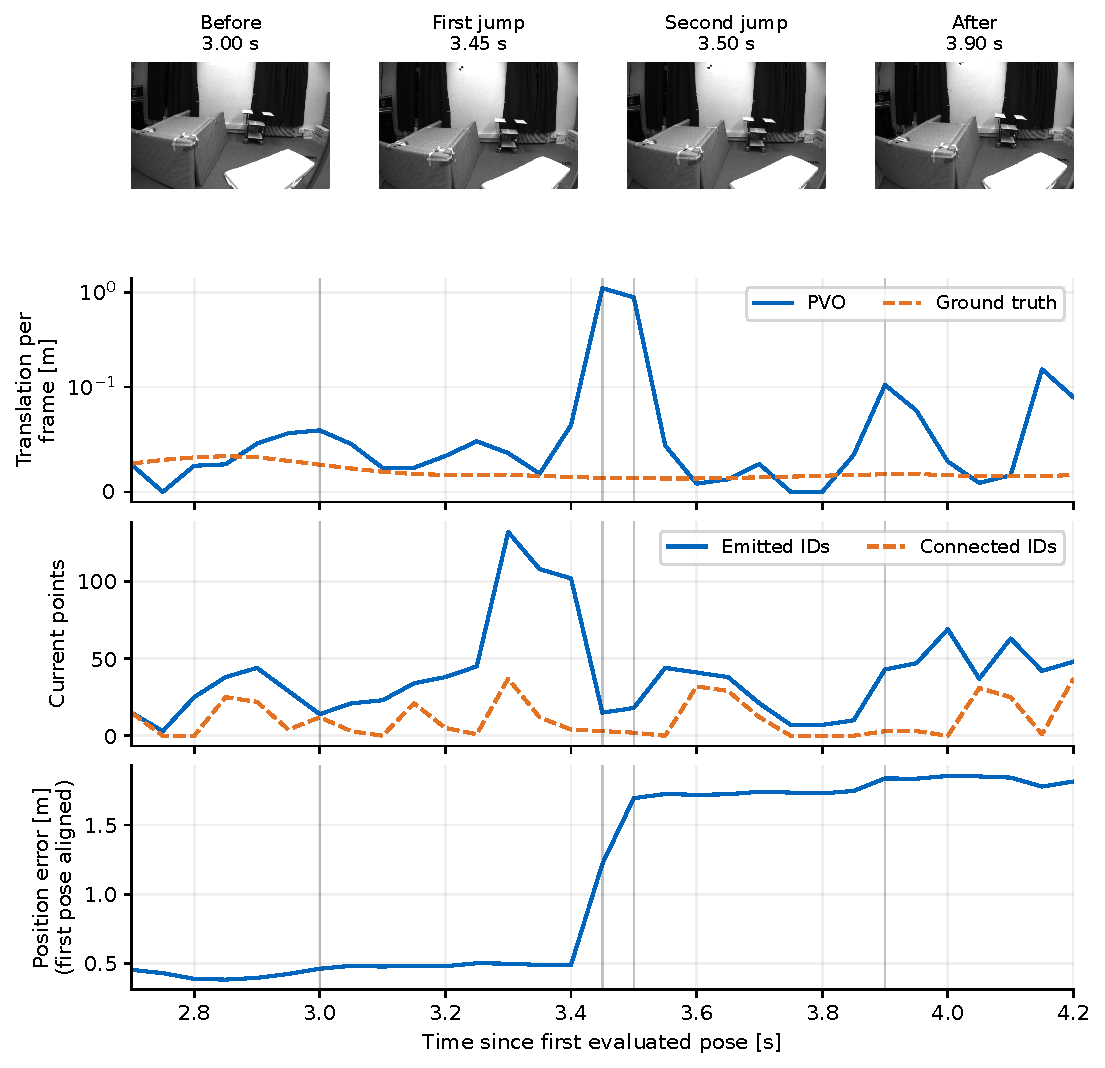
\includegraphics[width=\textwidth]{figures/evaluation/failure-ev202-early-jumps}
  \caption[Large translation estimates during small motion on EV202]{EV202's consecutive large translation estimates during small
  ground-truth motion. The native views change little across the updates, while
  only a few emitted IDs connect to existing landmarks. The position error uses
  first-pose alignment and is not globally aligned ATE.}
  \label{fig:failure-ev202-early}
\end{figure}

\begin{figure}[p]
  \centering
  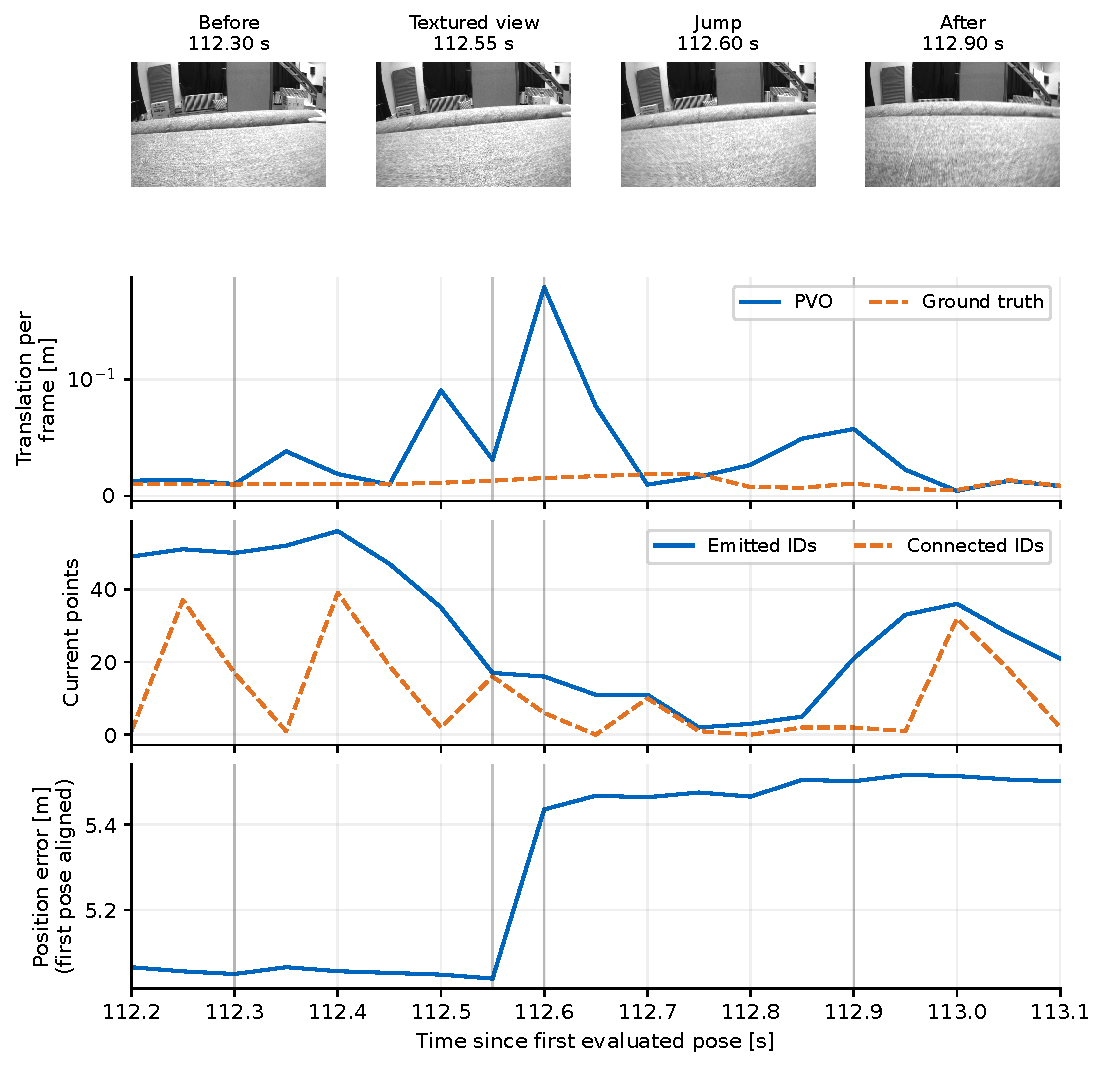
\includegraphics[width=\textwidth]{figures/evaluation/failure-ev202-textured-jump}
  \caption[EV202 failure despite abundant image texture]{An EV202 failure despite abundant visible texture. The jump frame
  contains 1640 offline Shi-Tomasi corners but only six IDs connected to existing
  landmarks. Estimated translation is \SI{0.752}{\metre}, compared with a
  ground-truth step of \SI{0.015}{\metre}. High image corner count is therefore
  not sufficient to establish usable geometric support.}
  \label{fig:failure-ev202-textured}
\end{figure}

\clearpage
\section{Full-Sequence Trajectories}\label{appendix:full-trajectories}

The following plots show PVO on all eleven EuRoC sequences, complementing the
examples in \autoref{sec:trajectory-geometry}.
Each pair of projections shows every saved PVO position after the single
whole-trajectory alignment used for ATE, together with the available reference
path. No scale correction, smoothing, or removal of failure segments is
applied. The axes use equal metric scale within a sequence and retain its full
extent. These spatial views complement, rather than replace, the timestamped
failure episodes.

EV202's estimated path is substantially distorted despite its small ATE
improvement over the stationary baseline. EMH04 retains broad excursions but
differs markedly in their geometry and vertical extent. EV103 contains a large
discontinuity far outside the reference path. Because alignment is fitted over
the complete sequence, this failure also shifts the earlier plotted estimates
relative to ground truth; their offset must not be interpreted as an initial
pose error.

\begin{figure}[p]
  \centering
  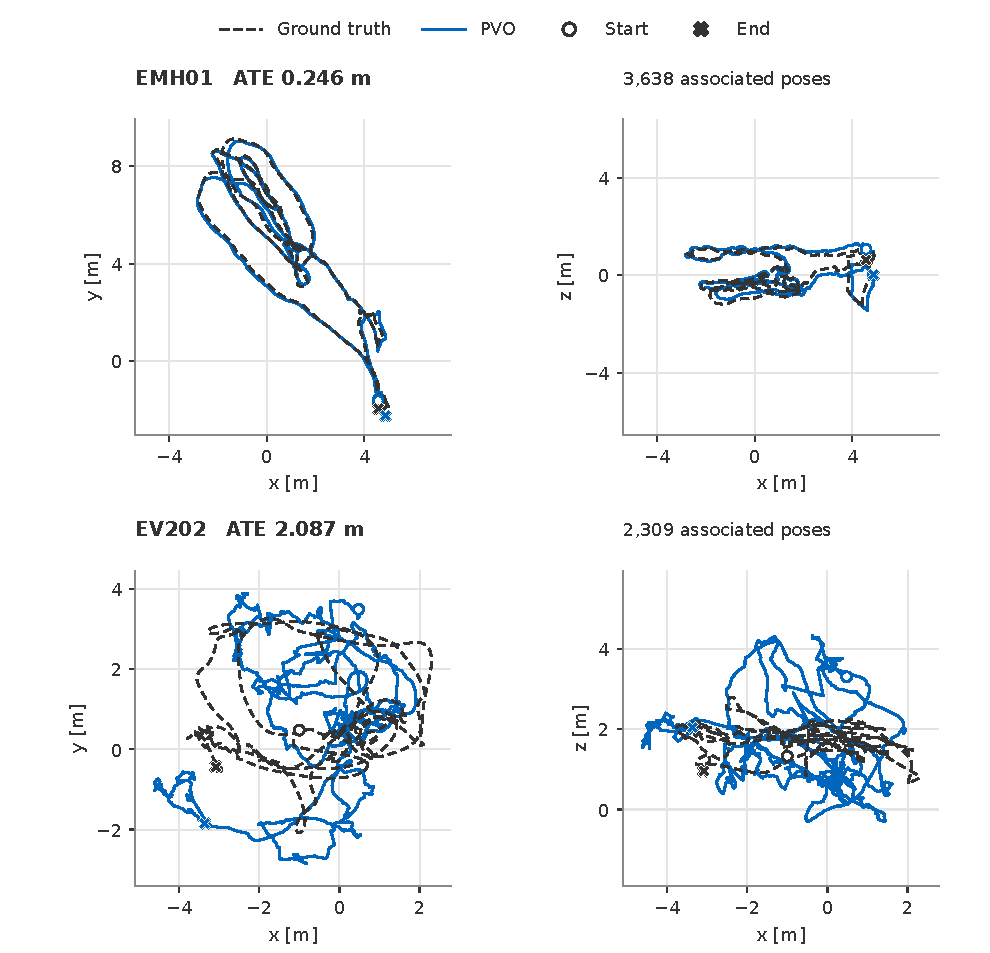
\includegraphics[width=\textwidth]{figures/evaluation/camera-trajectory-main-emh01-ev202}
  \caption[PVO trajectories on EMH01 and EV202]{Full-sequence PVO trajectories and ground truth for EMH01 and EV202,
  viewed in the $xy$ and $xz$ planes. Both views use the same rigid alignment
  as ATE, without scale correction. All saved estimates are shown; the pose
  counts identify those associated with ground truth for the reported metric.
  Circles and crosses mark the start and end of each displayed path.}
  \label{fig:trajectory-emh01-ev202}
\end{figure}

\begin{figure}[p]
  \centering
  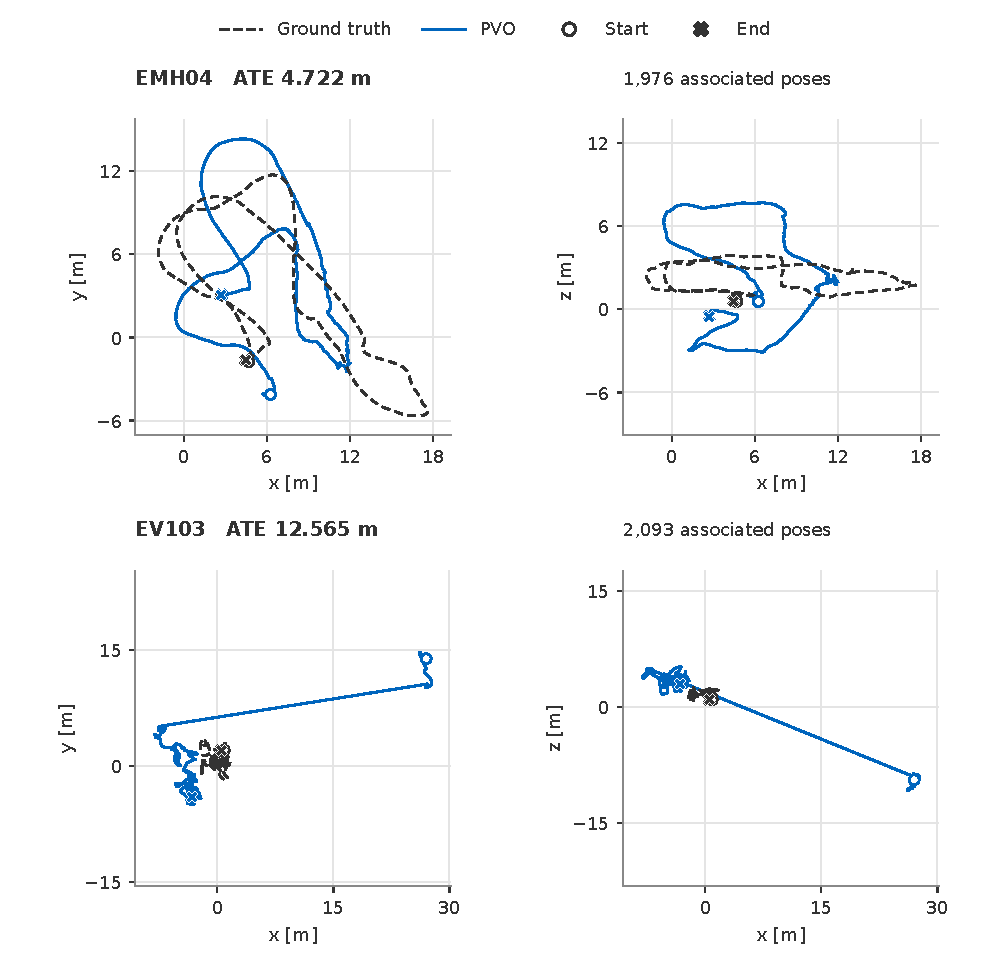
\includegraphics[width=\textwidth]{figures/evaluation/camera-trajectory-main-emh04-ev103}
  \caption[PVO trajectories on EMH04 and EV103]{Full-sequence PVO trajectories for EMH04 and EV103, using the same
  convention as \autoref{fig:trajectory-emh01-ev202}. The axes retain the full
  estimated extent, including EV103's catastrophic jump. Distances are equally
  scaled within each sequence, but axis ranges differ between sequences.}
  \label{fig:trajectory-emh04-ev103}
\end{figure}

\begin{figure}[p]
  \centering
  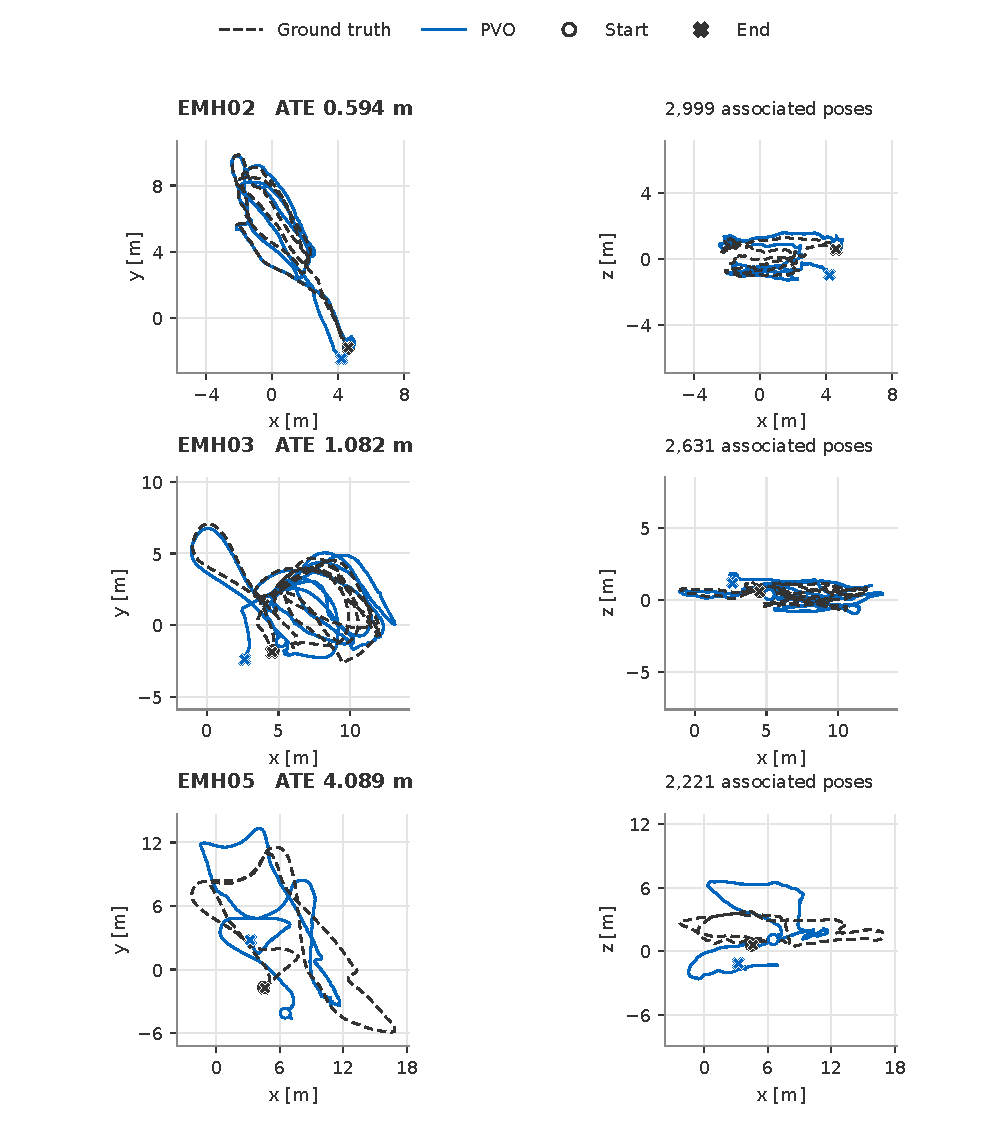
\includegraphics[width=\textwidth]{figures/evaluation/camera-trajectory-appendix-machine-hall}
  \caption[PVO trajectories on EMH02, EMH03, and EMH05]{Full-sequence PVO trajectories for the Machine Hall sequences
  EMH02, EMH03, and EMH05. Left: $xy$ projection; right: $xz$ projection.
  Circles and crosses mark the start and end of each displayed path.}
  \label{fig:trajectory-remaining-machine-hall}
\end{figure}

\begin{figure}[p]
  \centering
  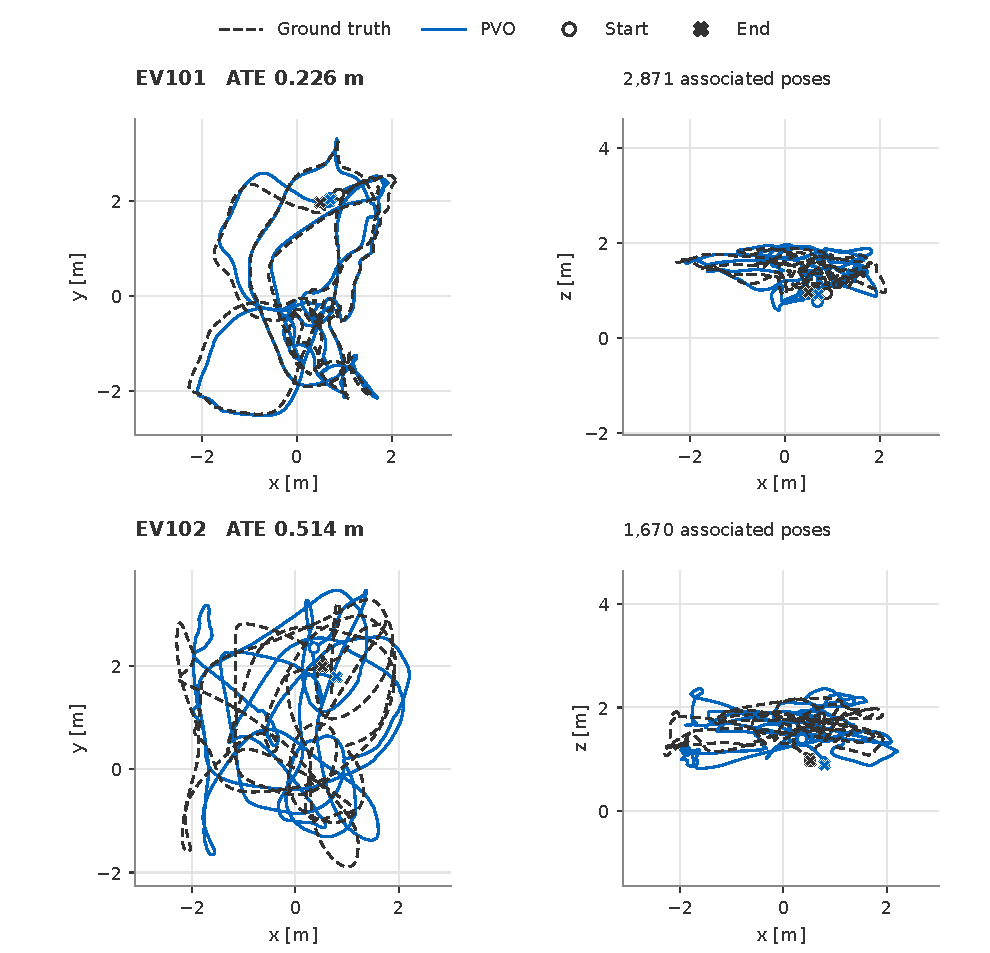
\includegraphics[width=\textwidth]{figures/evaluation/camera-trajectory-appendix-vicon-1}
  \caption[PVO trajectories on EV101 and EV102]{Full-sequence PVO trajectories for EV101 and EV102, using the same
  alignment and plotting convention as \autoref{fig:trajectory-emh01-ev202}.}
  \label{fig:trajectory-remaining-vicon-1}
\end{figure}

\begin{figure}[p]
  \centering
  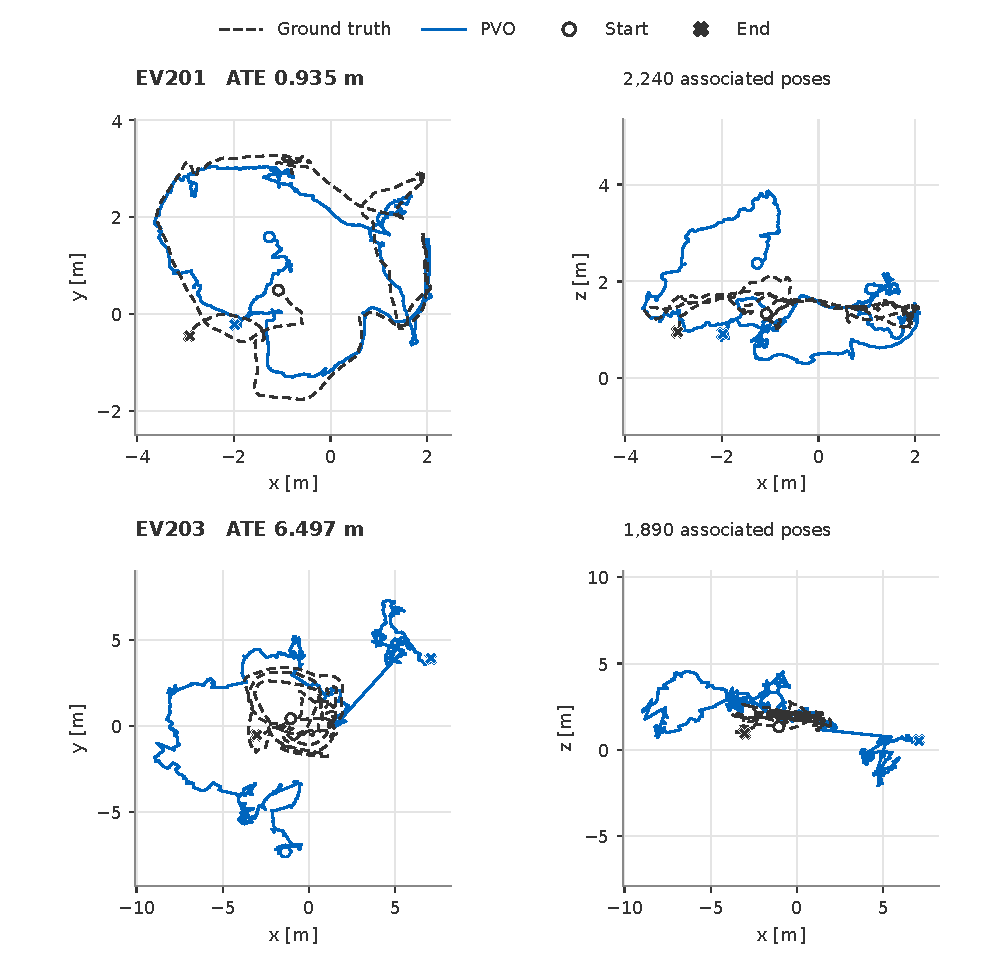
\includegraphics[width=\textwidth]{figures/evaluation/camera-trajectory-appendix-vicon-2}
  \caption[PVO trajectories on EV201 and EV203]{Full-sequence PVO trajectories for EV201 and EV203. The full extent of
  EV203's estimated motion is retained despite its much smaller reference path.}
  \label{fig:trajectory-remaining-vicon-2}
\end{figure}


\clearpage
\section{Stereo Transform Overview}\label{appendix:stereo-transforms}

The full set of twelve transformed encodings is illustrated on a later EMH02
stereo pair in \autoref{fig:stereo-all-shifts}. The rows vary disparity
pre-shift and the columns vary grid phase. This overview complements the
sampling construction and the location-specific recovery examples in
Chapter~\ref{chapter:method}.

\begin{figure}[htbp]
  \centering
  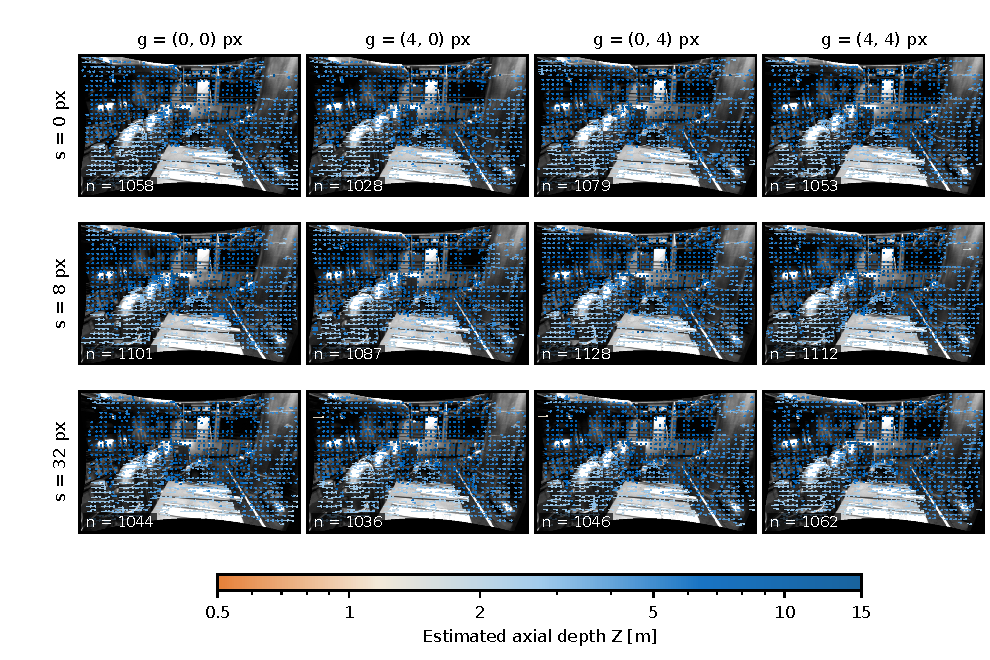
\includegraphics[width=\textwidth]{figures/method/stereo-all-shifts-late-emh02.pdf}
  \caption[Stereo correspondences across all twelve shifts]{All twelve stereo transforms for EMH02 at \SI{135}{\second}
  (pair 2700, zero based). Rows vary pre-shift $s$ and columns vary common
  grid phase $g$. Dots mark left-image locations; segments end at their
  right-image coordinates in the common rectified plane. Every
  positive-disparity observation surviving the diagnostic stereo checks is
  shown, with count $n$. Colour encodes estimated axial depth, clipped to
  the displayed \SIrange{0.5}{15}{\metre} scale.}
  \label{fig:stereo-all-shifts}
\end{figure}

% !TeX root = ../main.tex

\clearpage
\section{Lessons from Preliminary Experiments}\label{appendix:prior-experiments}

Several approaches preceded the stereo-depth alignment method developed in
this thesis. They explored filtering codec motion, using it to propagate
existing image features, and changing the lifetime or placement of tracked
samples. The examples below come from archived development experiments on
Monado sequences~\cite{deMayoCremersPireMSD}. Some used image features, inertial
rotation, or ground-truth geometry to investigate particular limitations; they
are separate from the final pixel-free EuRoC evaluation. Their common lesson
is that useful local motion and persistent point identity are distinct
requirements.

\subsection{Frequency-Based Selection of Motion Vectors}

An early idea was to distinguish coherent camera-induced motion from irregular
codec predictions through their frequency content. Motion-vector fields were
sampled on an eight-pixel grid and decomposed into spatial or spatiotemporal
frequency bands. A complementary temporal diagnostic compared successive
fields after alignment using the coded displacements. For two aligned motion
samples $\mathbf{m}_a$ and $\mathbf{m}_b$, the normalized two-point Fourier
transform has coefficients
\begin{equation}
  \frac{\mathbf{m}_a+\mathbf{m}_b}{2}
  \quad\text{and}\quad
  \frac{\mathbf{m}_a-\mathbf{m}_b}{2}.
\end{equation}
The second coefficient measures disagreement between the samples. A small
value suggests temporal consistency, but can also occur when both samples
share an incorrect displacement. A three-dimensional FFT over the two-frame
volume additionally measures spatial variation.

The diagnostic assigned each vector to the frequency band with the largest
reconstructed magnitude, provided that band's share of the summed magnitudes
exceeded a chosen dominance threshold. Spatial and spatiotemporal bands used
normalized radial cuts of 0.12 and 0.35.

\begin{figure}[!htbp]
  \centering
  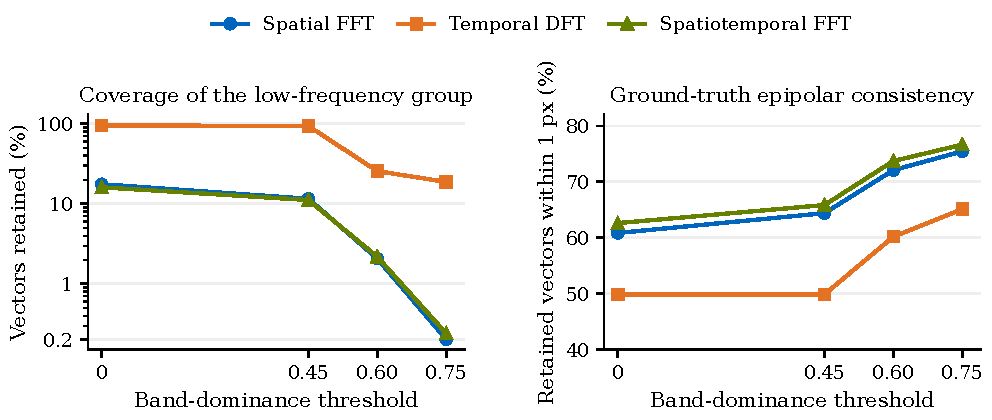
\includegraphics[width=\textwidth]{figures/appendix/prior-fft-coverage-consistency}
  \caption[Frequency selection: coverage and epipolar consistency]{Low-frequency
  selection on MOO06. Coverage uses a logarithmic axis. Consistency measures
  the fraction of retained vectors with ground-truth square-root Sampson
  residual at most one pixel, evaluated in undistorted coordinates and scaled
  by $\sqrt{f_xf_y}$. Spatial grouping covers 7,108,462 vectors; the temporally
  aligned methods cover 7,017,517 because they require a preceding field.}
  \label{fig:prior-fft-selection}
\end{figure}

\autoref{fig:prior-fft-selection} shows the resulting trade-off on MOO06.
At a threshold of 0.45, the spatiotemporal low-frequency group retained
11.15\% of the input vectors; 65.85\% of those satisfied the one-pixel
ground-truth epipolar check. Raising the threshold to 0.75 increased that
fraction to 76.65\%, but retained only 0.24\% of the vectors. Frequency
selection could therefore enrich a geometrically consistent subset at a
substantial cost in coverage. Even a small epipolar residual does not
establish the correct endpoint along the epipolar line or the identity of a
physical scene point.

A later variant ranked blocks by the sum of their reconstructed band
magnitudes and selected up to ten translation-support correspondences from
low-ranked blocks containing active features, for an inertial-rotation-assisted
epipolar filter. This score was called ``energy'' during development, although
it was not squared Fourier energy. Without image refinement of these
supports, global ranking produced \SI{0.538}{\metre} ATE RMSE on the full
4,171-frame MOO06 run, compared with
\SI{0.177}{\metre} for image-refined translation support. Selecting supports
within spatial windows improved the ranked variant to
\SI{0.299}{\metre}. These run-level results evaluate support sets, not the pose
consistency of the single lowest-scoring vector; they therefore do not settle
the latter question.

\subsection{Propagating Existing Features}

Another approach retained the identities of existing image features and
propagated their coordinates with codec displacements. At each transition,
it selected a motion vector whose source support contained the current
feature location, applied that vector, and stored the endpoint under the
same track ID. The attraction was to reuse an established feature-based
backend while replacing repeated temporal image matching. However, carrying
an ID forward does not verify that its new coordinate still observes the
same physical point.

\autoref{fig:prior-mv-propagation} illustrates the difference between a
promising short run and sustained tracking on MIO07. The archived direct-MV
prototype reached approximately \SI{0.096}{\metre} ATE over its first 800
frames, but approximately \SI{30.27}{\metre} over the full 4,095-frame
sequence. The image-based reference finished at approximately
\SI{0.120}{\metre}. The prototype still assigned vectors to 92.8\% of
attempted feature propagations. That count describes available assignments,
not their geometric correctness or preservation of point identity.

\begin{figure}[htbp]
  \centering
  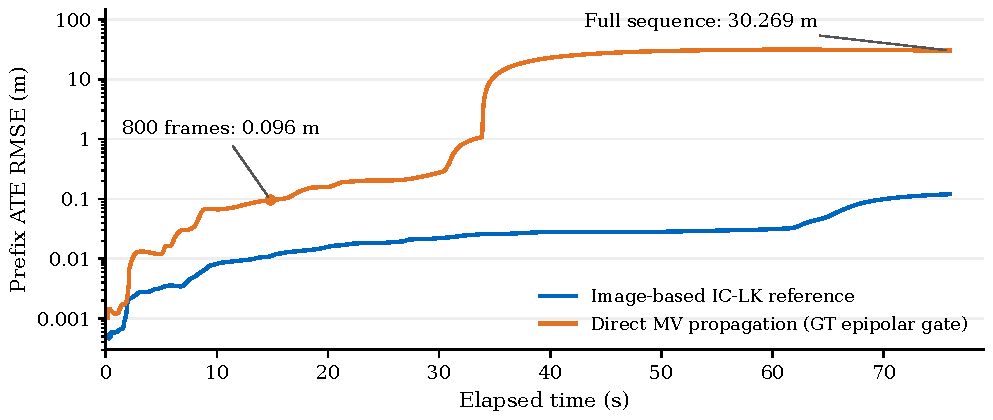
\includegraphics[width=\textwidth]{figures/appendix/prior-mv-propagation-prefix-error}
  \caption[An early direct-MV propagation failure]{Archived MIO07 development
  run: direct temporal MV propagation and an image-based inverse-compositional
  Lucas--Kanade reference. Each plotted ATE is evaluated over the prefix ending
  at that time, with a new rigid alignment and fixed scale for that prefix.
  The vertical axis is logarithmic. The direct-MV prototype used a
  ground-truth epipolar gate with a loose 32-pixel threshold, retaining
  99.6\% of input vectors; it was not an oracle for correct point identity.
  Image-based feature detection and stereo matching were retained; codec
  vectors replaced temporal tracking only.
  The curves are redrawn from the archived per-prefix measurements and do not
  represent the final PVO configuration.}
  \label{fig:prior-mv-propagation}
\end{figure}

This failure does not isolate identity drift as its sole cause: geometric
support, stereo observations, and backend conditioning also matter. It shows
why short-prefix accuracy and high assignment counts were insufficient
validation. The feature-seeded diagnostic in
\autoref{fig:mv-feature-departure-example} shows a local mechanism: codec
propagation can depart from an image track despite a common starting point
and continuing vector support.

\FloatBarrier
Further tests examined feature placement and temporal connectivity
separately. In a stereo-inertial test with spatial refill opportunities
controlled, using arbitrary codec block centres as starting locations
reduced successful temporal KLT
counts to 35.8\% of the FAST-location reference on MIO07 and 37.1\% on
MOO07. This experiment retained image-based tracking and did not use codec
displacements; it showed that block centres were not interchangeable with
selected image features. In a separate visual-only stereo test on 800 MIO07 frames using KLT
correspondences, restricting landmarks to adjacent frame pairs produced
\SI{0.521}{\metre} ATE. Making every frame a keyframe improved this to
\SI{0.035}{\metre}, while persistent tracks achieved
\SI{0.011}{\metre}. Shorter identities therefore also required changes to
landmark admission and map connectivity; they were not a complete solution
on their own.

\subsection{Persistent Surfaces with Changing Point Support}

These observations suggest a direction beyond improving a point-selection
rule. The useful codec support on an extended surface can change from frame
to frame. For example, observations on a tabletop might shift between its
edge, a corner, and an interior textured region. Such observations may remain
compatible with the motion of the same static surface even when they cannot
be joined into one long-lived point track. This is a motivation for testing
surface-level association, not evidence that the present experiments already
recover object identities.

Li and Song~\cite{li2014toward} provide a relevant precedent under a planar
scene model. They group codec correspondences using homography RANSAC,
associate planes across frames, and jointly estimate plane geometry and
camera motion in an extended Kalman filter. Their state can retain a plane
while its supporting point correspondences change. The observation model
still uses those correspondences through a plane-induced homography; the
plane label alone does not supply camera motion.

A future codec-based estimator could similarly maintain a static plane or
other geometric region while renewing its short-lived correspondence support.
It would need reliable region association, enough spatially distributed
observations, and geometry that constrains the camera motion. Merely seeing
another part of the same object would not satisfy these requirements.
Non-planar objects would require an appropriate shape or rigid-body model,
and independently moving objects would need separate treatment. Preserving
the pixel-free boundary would also require forming and associating these
regions from codec metadata and geometry. The stereo-depth construction in
this thesis supplies one possible source of that geometry; whether a surface
representation makes better use of intermittent codec support remains an
open experimental question.

